\documentclass[11pt]{article}
\usepackage{amsmath,amsthm,amssymb,fullpage,graphicx,hyperref,listings}
\usepackage{listings,color,setspace}
\author{Andy Reagan}
\title{Math 337 Homework 07}

     \def\NN{\mathbb{N} }
     \def\ZZ{\mathbb{Z} }
     \def\QQ{\mathbb{Q} }
     \def\RR{\mathbb{R} }
     \def\CC{\mathbb{C} }
     \def\f{\frac }
     \def\b{\begin }
     \def\e{\end }
     \def\Log{\text{Log} \,}
     \def\Re{\text{Re} \, }

\lstset{language=MATLAB,
basicstyle=\ttfamily\scriptsize\singlespacing,
keywordstyle=\color{blue},
stringstyle=\color{red},
commentstyle=\color{green},
morecomment=[l][\color{magenta}]{\#},
frame=L,
xleftmargin=\parindent,
%%numbers=left,                   %% where to put the line-numbers
%%numberstyle=\scriptsize,      %% the size of the fonts that are used for the line-numbers
%%stepnumber=1,                   %% the step between two line-numbers. If it is 1 each line will be numbered
numbersep=5pt,
breaklines=true,        %% sets automatic line breaking
breakatwhitespace=false,    %% sets if automatic breaks should only happen at whitespace
escapeinside={\%*}{*)} 
}


     \newcommand{\pdiff}[2]{\frac{\partial #1}{\partial #2}}
     \newcommand{\partialdiff}[2]{\frac{\partial #1}{\partial #2}}
     \newcommand{\pdiffsq}[2]{\frac{\partial^2 #1}{{\partial #2}^2}}
     \newcommand{\pdiffcu}[2]{\frac{\partial^3 #1}{{\partial #2}^3}}
     \newcommand{\pdiffhi}[3]{\frac{\partial^#3 #1}{{\partial #2}^#3}}
     \newcommand{\diff}[2]{\frac{{\rm d}#1}{{\rm d}#2}}
     \newcommand{\diffsq}[2]{\frac{{\rm d}^{2}#1}{{\rm d} {#2}^2}}
     \newcommand{\diffhi}[3]{\frac{{\rm d}^#3 #1}{{\rm d} {#2}^#3}}
     \newcommand{\tdiff}[2]{\mbox{d} #1/\mbox{d} #2}
     \newcommand{\tdiffsq}[2]{\mbox{d}^{2} #1/\mbox{d} {#2}^2}
     \newcommand{\tpdiff}[2]{\partial #1/\partial #2}
     \newcommand{\tpdiffsq}[2]{\partial^2 #1/\partial {#2}^2}
     \newcommand{\bvec}[1]{\vec{ {\bf #1 } }}
     \newcommand{\oh}[1]{O(h^{{#1}})}

\begin{document}
\maketitle

\begin{enumerate}

\item Solve the BVP
\[ y'' + xy' - 3y = 3x, y(0) = 1, y(2) = 5 \]
by the shooting method.
Use the modified Euler method with $h = 0.1$ as the IVP solver.
Plot your solution.

\bigskip
\textbf{Solution:} My code and a solution plot follow.

\lstinputlisting[language=Matlab]{andy_hw07_prb01.m}

\begin{figure}[h!]
  \centering
    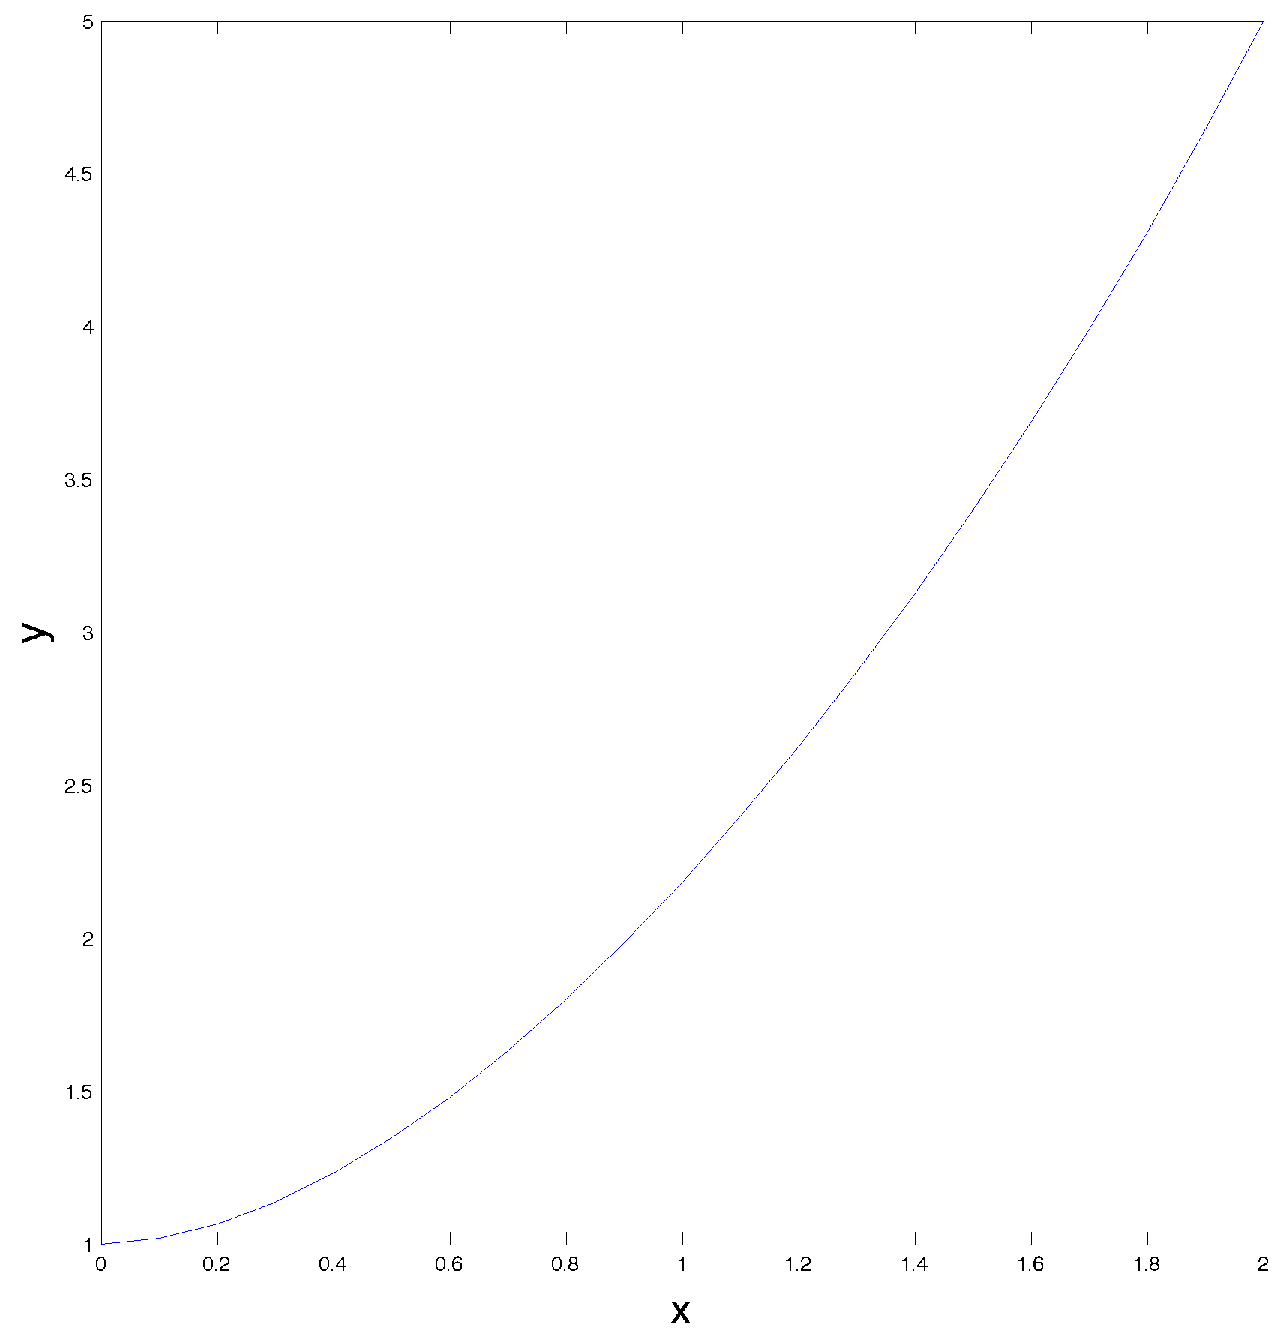
\includegraphics[width=0.5\textwidth]{andy_hw07_prb01_01.pdf}
  \caption{Solution of the BVP with the shooting method.}
\end{figure}

\item Solve the BVP
\[ x^3 y''' + xy' -y = -3 + \ln x, y(1) = 1, y'(2) = 1/2, y''(2) = 1/4 \]
by ``shooting'' from the left end point and using the example given in the notes.
Use the ME method with $h = 0.02$.
Plot your solution

\bigskip
\textbf{Solution:} My code and a solution plot follow.

\lstinputlisting[language=Matlab]{andy_hw07_prb02.m}

\begin{figure}[h!]
  \centering
    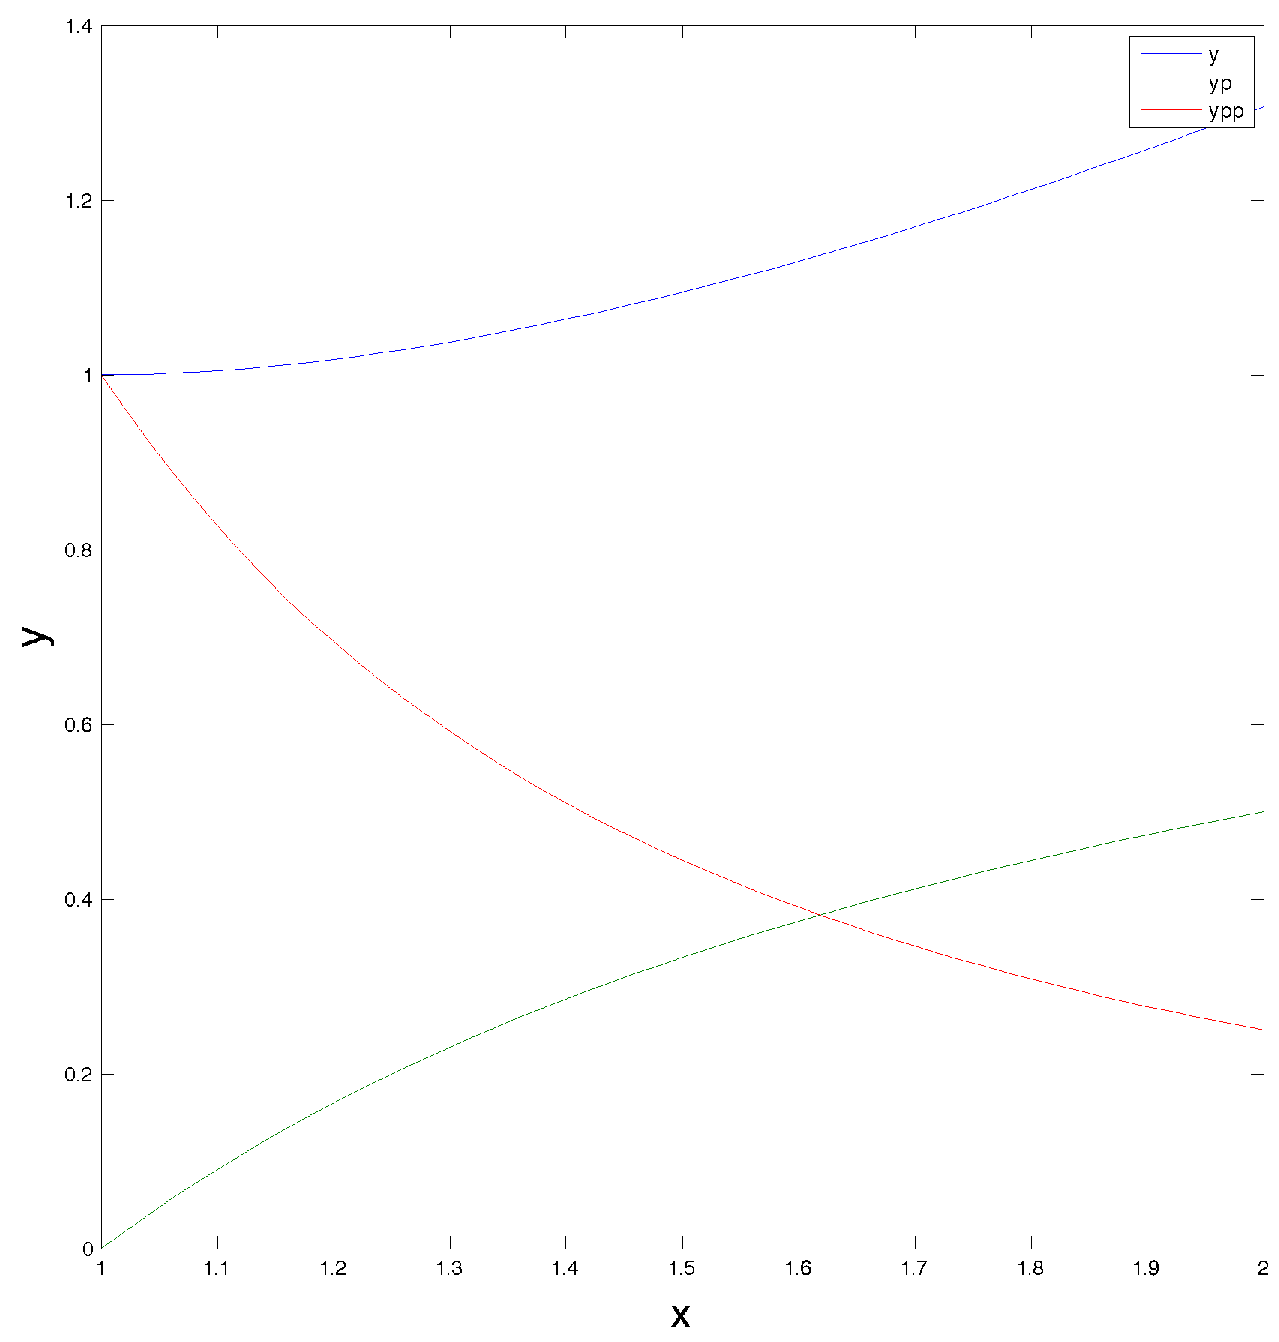
\includegraphics[width=0.5\textwidth]{andy_hw07_prb02_01.pdf}
  \caption{Solution of the BVP with the shooting method. Here yp denotes $y'$ and ypp denotes $y''$.}
\end{figure}

\item Solve problem 2, in reverse.

\bigskip
\textbf{Solution:} My code and a solution plot follow.
I found it easiest to write a ME function that goes backwards.

\lstinputlisting[language=Matlab]{andy_hw07_prb03.m}

\begin{figure}[h!]
  \centering
    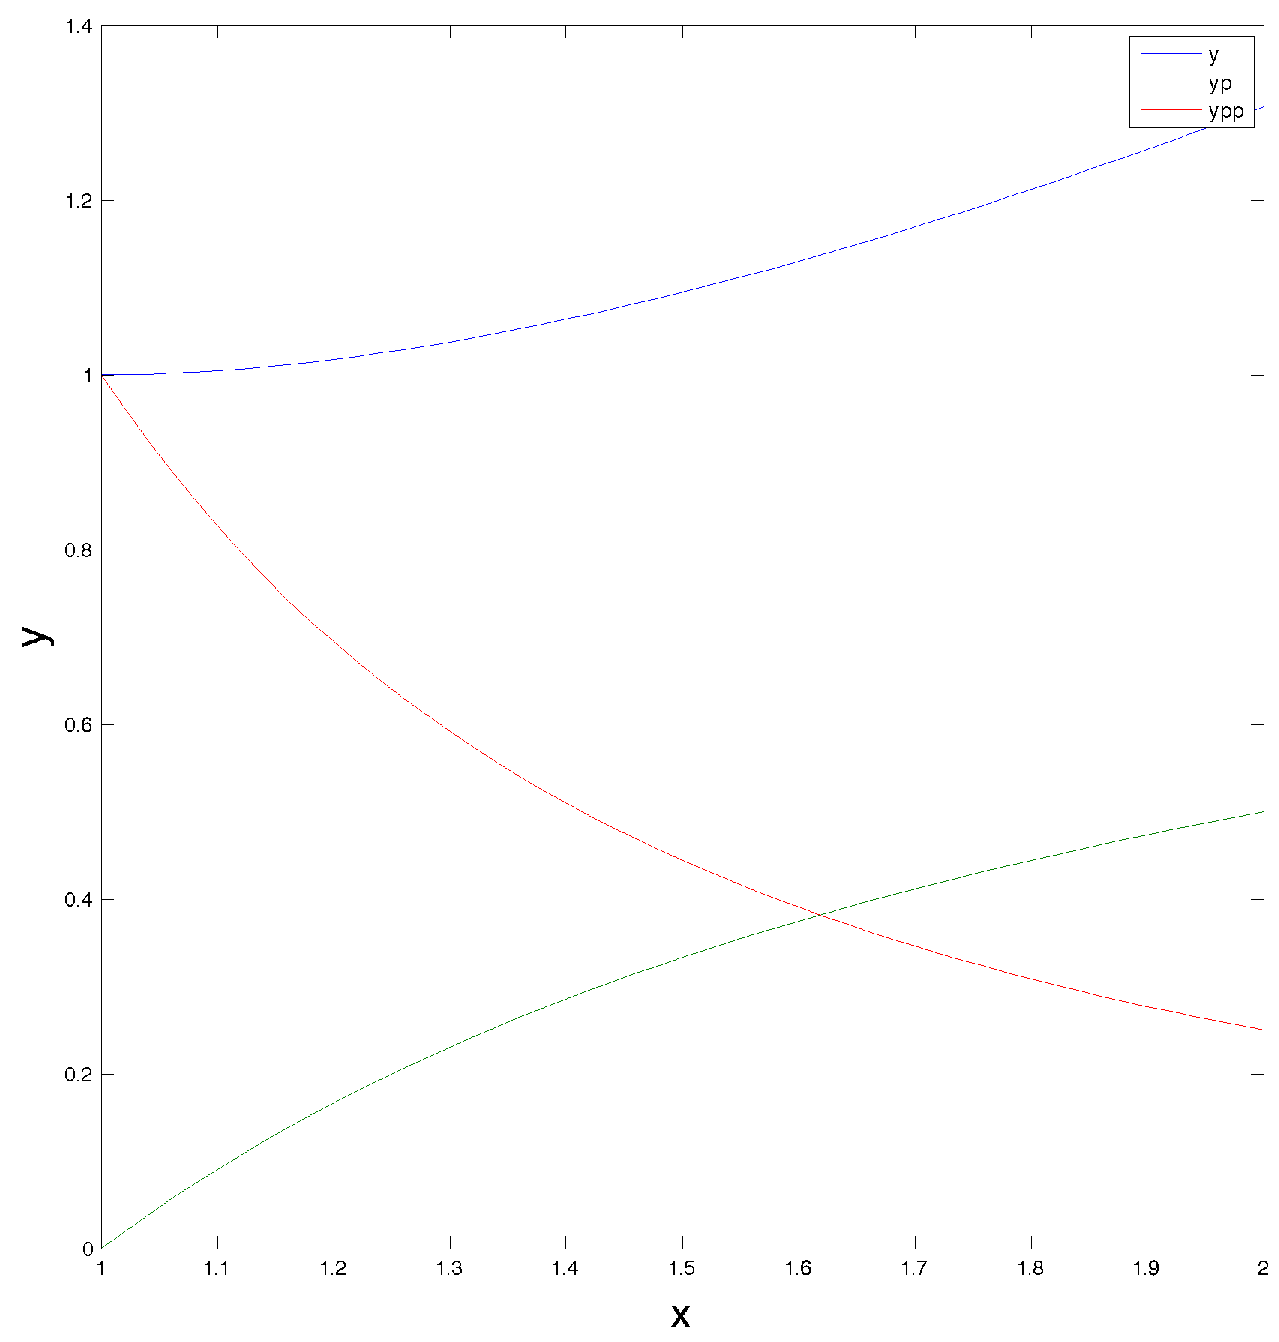
\includegraphics[width=0.5\textwidth]{andy_hw07_prb03_01.pdf}
  \caption{Solution of the BVP with the shooting method. Here yp denotes $y'$ and ypp denotes $y''$.}
\end{figure}

\begin{align*} \end{align*}

\end{enumerate}

%% \begin{figure}[h!]
%%   \centering
%%     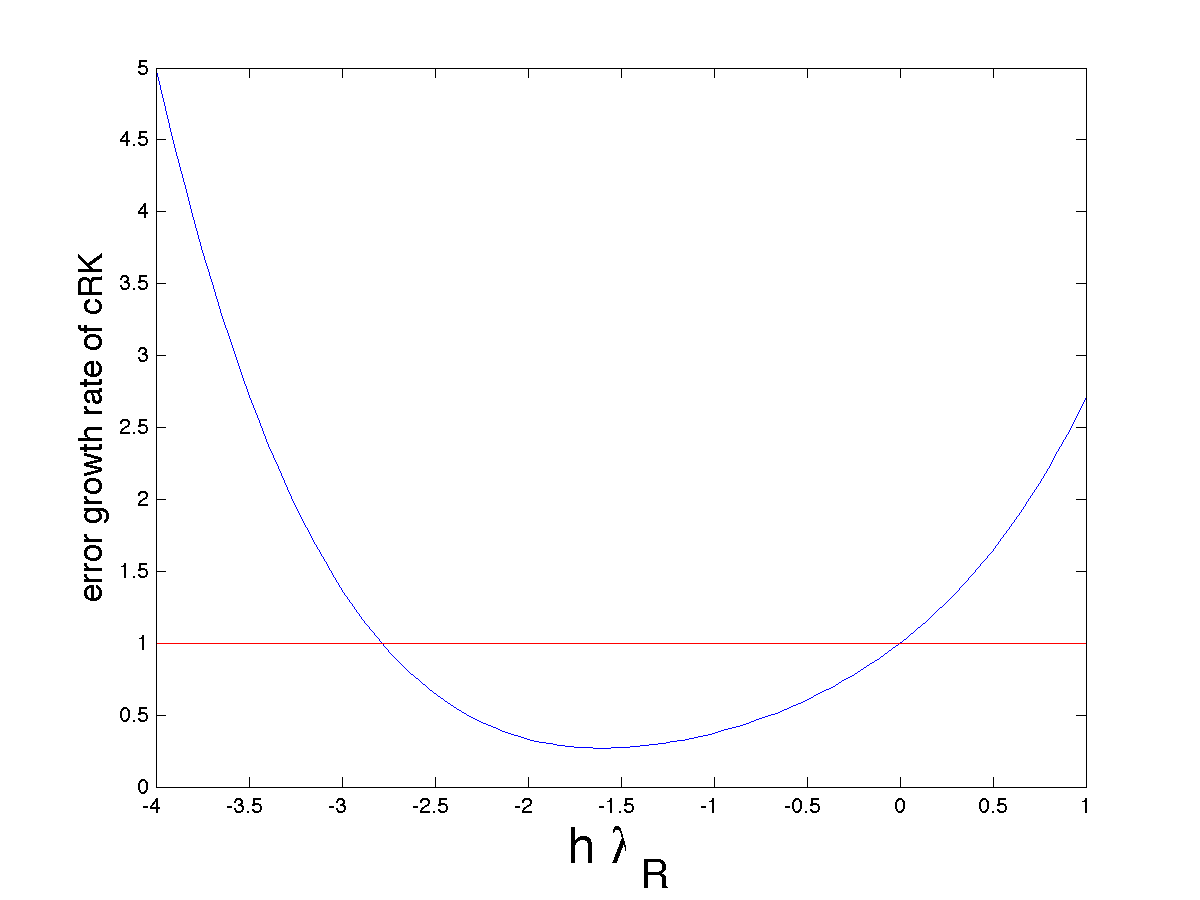
\includegraphics[width=0.5\textwidth]{andy_hw04_prb02_01.png}
%%   \caption{Stability of the cRK method.}
%% \end{figure}

%% \lstinputlisting[language=Matlab]{andy_hw04_prb04.m}

\end{document}
